\documentclass[letter, 11pt]{article}
\usepackage[utf8]{inputenc}
\usepackage[spanish]{babel}
\usepackage{amsfonts}
\usepackage[dvips]{graphicx}
\usepackage{url}
\usepackage{graphicx} %Permite exportar imagenes en formato eps
\usepackage{url} %Tipo de fuente para correos y paginas
\usepackage{pgf}
\usepackage{fleqn}
\usepackage{amssymb}
\usepackage{amsmath}
\usepackage{fancyvrb}
\usepackage{makeidx}
\usepackage{colortbl} %Permite colocar colores a las tablas
\usepackage{multirow}
\usepackage{booktabs}
\usepackage{moreverb}
\usepackage{rotating}
\usepackage[final]{pdfpages}

\usepackage[top=3cm,bottom=3cm,left=3.5cm,right=3.5cm,footskip=1.5cm,headheight=1.5cm,headsep=.5cm,textheight=3cm]{geometry}

\begin{document}
\title{Inteligencia Artificial \\ \begin{Large}Estado del Arte: Problema \textit{Aircraft Landing Scheduling}\end{Large}}
\author{Victor Gonzalez Rodriguez\\ \url{victor.gonzalezro@alumnos.usm.cl}}
\date{\today}
\maketitle


%--------------------No borrar esta secci\'on--------------------------------%
\section*{Evaluación}

\begin{tabular}{ll}
Resumen (5\%): & \underline{\hspace{2cm}} \\
Introducci\'on (5\%):  & \underline{\hspace{2cm}} \\
Definici\'on del Problema (10\%):  & \underline{\hspace{2cm}} \\
Estado del Arte (35\%):  & \underline{\hspace{2cm}} \\
Modelo Matem\'atico (20\%): &  \underline{\hspace{2cm}}\\
Conclusiones (20\%): &  \underline{\hspace{2cm}}\\
Bibliograf\'ia (5\%): & \underline{\hspace{2cm}}\\
 &  \\
\textbf{Nota Final (100\%)}:   & \underline{\hspace{2cm}}
\end{tabular}
%---------------------------------------------------------------------------%
\vspace{2cm}


\begin{abstract}
En este informe, consideramos el problema de Aircraft Landing Scheduling, donde se modela el aterrizaje de aviones en distintas pistas de un aeropuerto. Este problema nos ayuda a decidir el tiempo y lugar donde un avión debería aterrizar dentro de una ventana predeterminada de tiempo, respetando la separación de tiempo entre aterrizajes y la secuencia respectiva de aviones que deben aterrizar después. Analizaremos el estado del arte de los métodos actualmente publicados, de manera que se genere una idea general de las implementaciones disponibles para resolver este problema, y analizar así cuales son los mejores acercamientos y sus evoluciones. Finalmente, esto se presentará mediante un modelo matemático, formulando sus respectivas restricciones y variables, para luego comentar y concluir el estado del arte al presente año.
\end{abstract}

\begin{description}
\item[Keywords:] Aircraft Landing Scheduling problem, estado del arte, modelo matemático, calendarización de aterrizajes, Aircraft Arrival and Departure Sequencing problem.
\end{description}
\newpage

\section{Introducción}
El Aircraft Landing Scheduling Problem (ALSP), o \textit{Problema de Calendarización de Aterrizaje de Aeronaves} en español, es un problema que ha ganado mucha importancia a nivel mundial, especialmente los últimos años debido a la gran congestión de aviones que están circulando actualmente en el espacio aéreo mundial, y la necesidad de mantener el flujo de aeronaves lo más fluido posible sin perder de vista la seguridad de los pasajeros que son parte escencial de todo este sistema. Ejemplo de esto es la investigación impulsada gubernamentalmente en el aeropuerto de Heathrow hace un par de años atrás [2].

El ALSP es catalogado como un problema muy complejo, el cual en la clasificación estándar, se lo cataloga como NP-complejo\footnote{Tan complejo como el más dificil de los problemas polinomiales no-deterministas.}, y debido a esto mismo, las implementaciónes disponibles en las publicaciones a nivel mundial, pueden llegar a ser muy complejas y difíciles de entender. Debido a esta situación, hemos de entregar una definición del problema que sólo involucre los factores más comunes y/o significativos para modelar el ALSP, y a partir de esto, se presentará un modelo matemático tan sencillo como la definición del problema lo permita.

Estudiaremos ademas, las distintas implementaciones disponibles actualmente de manera superficial, de modo que se pueda comparar a grandes rasgos cual es la tendencia mundial o histórica para resolver este tipo de problemas, situando al lector en la situación actual de la modelación de estos problemas.

A partir de lo presentado previamente en este documento, se comentará, justificará y comentará lo expuesto en la sección llamada \textit{Estado del Arte} y \textit{Modelo Matemático}.

Finalmente, es de esperar que la información entregada en este documento, sea de ayuda para tener una buena noción de lo que está ocurriendo actualmente respecto al ALSP, y cuales serían los mejores acercamientos para resolver este tipo de problemas en la actualidad.

\section{Definición del Problema}
Debido a la creciente demanda de vuelos al rededor del mundo durante las últimas décadas, junto con el impulso de la tecnología y el explosivo aumento de pasajeros, ha puesto a los aeropuertos manejando cientos viajes en un día. Todo esto sin dejar de lado la seguridad, los tiempos de despegue/aterrizaje y la optimización del uso de los recursos de infraestructura.

Para darnos una idea gráfica del tráfico actual en el mundo, disponemos de la siguiente captura del día viernes 10 de mayo de 2013 a las 19:00 horas aproximadamente.
\begin{figure}[!h]
\centering
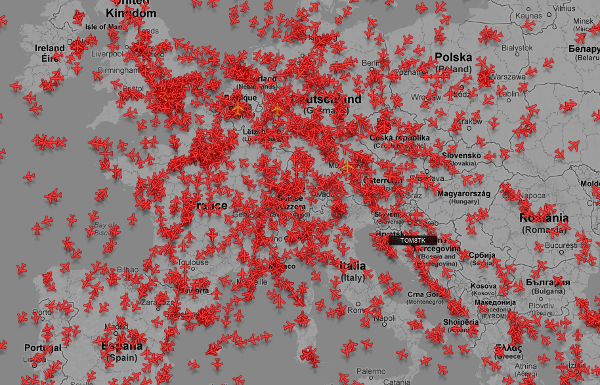
\includegraphics[width=9cm]{aviones.png}
\centering
\caption{fuente: http://www.planefinder.net/}
\end{figure}

El ALSP modela la situación de aeropuertos, aeródromos, bases militares y portaaviones, los cuales desde este momento los llamaremos simplemente como \textit{aeropuertos}, donde se quiere aterrizar, los cuales se llamarán a partir de ahora \textit{aterrizajes}, englobando también a los despegues, ya que en la práctica, no existe mucha diferencia entre ambos; despegar o aterrizar es simplemente hacer uso de una de las pistas del aeropuerto en una ventana de tiempo determinado.

En la instancia que analizaremos de este problema, abordarémos la situación de un aeropuerto con $n$ pistas y con un listado estático de aterrizajes, donde se sabe explicitamente y sin cambios, cuales serán las franjas de tiempo donde deben aterrizar los aviones entre sus muchas otras variables necesarias para describir el aterrizaje, el cual es la entrada del modelo matemático. El problema por el cual surge este problema, es que los vuelos están sujetos a retrasos, ya sea debido a variables atmosféricas, fallas técnicas de los aviones, daños durante el vuelo, etc. Todos estos problemas son propensos a retrasar el aterrizaje de un avión, afectando además a las demas naves. Es por esto que es necesario calendarizar de manera óptima los vuelos, de modo que se disponga de los tiempos óptimos para el aterrizaje considerando todos los eventos externos que pueden retrasar un vuelo, sin afectar el posible alto flujo de aterrizajes que se deben producir.

Para entrar en detalle, definiremos los aspectos más relevantes que pueden complicar la calendarización de los aterrizajes, los cuales obligarán al orden tomar en cuenta no solo el tiempo de llegada y las pistas disponibles:

\begin{itemize}
\item \textbf{Carga de la nave:} Aviones con muchos pasajeros, llevan mucho más equipaje, por lo que el tiempo de carga/descarga y los chequeos de seguridad afectan directamente al personal del aeropuerto, el cual es limitado y debe tener bajos tiempos de respuesta para efectuar los trabajos respectivos.

\item \textbf{Velocidad de vuelo:} Durante el vuelo, los aviones tienen una velocidad crucero, la cual permite estimar con antelación sus aterrizajes. Si se altera esa velocidad crucero, implica un costo tanto por el uso de combustible, como para definir un aterrizaje.

\item \textbf{Combustible:} La cantidad de combustible define el tiempo máximo de vuelo de un avión, lo cual es relevante para definir la ventana de tiempo de espera, antes que un avión aterrize mientras espera un cupo.

\item \textbf{Turbulencia de despegue:} Los aviones más grandes, ya sean comerciales o militares, generan mucha turbulencia al momento de despegue o aterrizaje, por lo que se debe disponer de una ventana de tiempo entre aterrizajes para estos aviones, de manera que no afecten la aerodinámica de los que vienen después.
\end{itemize}

\section{Estado del Arte}


\subsection{Métodos Actuales}

\subsubsection{Algoritmos Genéticos}
Este tipo de algoritmos por un buen tiempo han estado en la punta de lanza para resolver problemas de optimización o calendarización. Por lo general, estos algoritmos son los más usados cuando se trata de resultados liberados en tiempo real, ya que tienen un muy baja incertidumbre respecto al largo de las operaciones [1].

Los algoritmos genéticos se pueden resumir mediane el siguiente pseudo-código:

\begin{verbatimtab}[4]
Inicializar población inicial
Repetir hasta terminar:
	Evaluar conveniencia (ej: costos, tiempo de viaje)
	Reducir la población
	Seleccionar pares entre las mejores opciones (fitness)
	Repoblar usando los pares
		Aplicar operador de cruce
		Aplicar operador de mutación
	Verificar criterio de término
		Limites de tiempo, minima conveniencia satisfecha, etc.
		Iterar si no se ha terminado
\end{verbatimtab}

De acuerdo a esto, ajustando el ALSP a este tipo de algoritmos nos damos cuenta, que contamos con una población de calenderizaciones potenciales y está siempre disponible, y mientras más se ejecute el algoritmo, aparecerán mejores soluciones, esto nos dice que en cualquier momento encontraremos nuestro óptimo.

Sin embargo, existe una variante de este algoritmo que interesantemente se asemeja a lo que nosotros necesitamos, la cual se llama \textit{seed modifier}, el cual hace que en cada mutación del algoritmo, no se parta sin aviones aterrizados (sin semillas), lo cual se puede lograr del siguiente modo:

\begin{verbatimtab}[4]
Población inicial: población restante del último problema
Repetir hasta terminar:
	Evaluar conveniencia (ej: costos, tiempo de viaje)
	Reducir la población: eliminar aviones que aterrizaron
	Seleccionar pares entre las mejores opciones
	Repoblar usando los pares: aviones que llegaron después
		Aplicar operador de cruce
		Aplicar operador de mutación
	Verificar criterio de término
		Limites de tiempo, minima conveniencia satisfecha, etc.
		Iterar si no se ha terminado
\end{verbatimtab}

Haciendo la analogía entre este algoritmo y ALSP, los genes representan el tiempo de aterrizaje y la pista de aterrizaje que les corresponde, donde se tiene una lista estática que puede ser consultada en cualquier momento para ejecutar las funciones de fitness o para repoblar el algoritmo, de manera que este algoritmo puede consultar por el tiempo de vuelo máximo de los aviones, la carga, cantidad de pasajeros, etc.

\subsubsection{Algoritmo evolutivo diferencial de búsqueda de vecinos}
Los algoritmos evolutivos tienen la característica de cumplir bien bajo la demanda de problemas de optimización de múltiples objetivos. Esto resulta especialmente útil cuando consideramos que por lo general, las restricciones impuestas por los modelos tienden a tener conflictos entre sí.

En este caso, el algoritmo busca optimizar 2 objetivos:
\begin{enumerate}
\item Costo asociado al aterrizaje.
\item Tiempo estimado de llegada (ETA: Estimated Time Arrival).
\end{enumerate}

Primero se define una secuencia de aterrizaje utilizando algún método de ordenamiento como PEPS\footnote{Primero en entrar, primero en salir, o FCFS (First Come, First Served) por sus siglas en inglés.}, o técnicas más complejas como NAR\footnote{Non-dominated Average Ranking, el cual consiste en un algoritmo indirecto y eficiente por lo rápido, y por lo conveniente de su sistema de ranking que provee.}. Luego de esto, se aplica el algoritmo evolutivo multiobjetivo llamado MONSDE\footnote{Muti-Objective Neighborhood Search Diferential Evolution} [7], el cual es el encargado de determinar finalmente la secuencia de aterrizaje para todos los aviones.

\subsubsection{Algoritmo evolutivo de manejo de restricciones}
Este algoritmo lidia de mejor manera respecto a las restricciones que nos entrega el ALSP. Tiene un parecido significativo respecto al Algoritmo Genético, pero su función es resolver los conflictos de las restricciones respecto a la función objetivo del problema. Su implementación es algo similar a esto:

\begin{verbatimtab}
Generación de Población Inicial
Repetir hasta terminar:
	Evaluar funcion objetivo
	Generar nueva población:
		Mutación/recombinación/selección
	Evaluar término
		Criterio de Tiempo, costo, etc. alcanzado
		Iterar si no ha terminado
\end{verbatimtab}

Este algoritmo puede encontrar una región relativamente desable dentro del espacio de búsqueda, de manera que entregue una calendarización para el problema. Todo esto depende de que tan bien se defina el manejo de las restricciones, ya que estas son el cuello de botella del algoritmo evolutivo. [8]

 \subsubsection{Método híbrido de resolución basado en formulación de Job Shop}
Se plantea una formulación del problema de aircraft landing scheduling estático con varias pistas de aterrizaje que contiene menor número de restricciones, lo que puede reducir el tiempo de computo), y luego se modela el mismo problema como si fuera un job shop scheduling, para mostrar la relación que existe entre ambas formulaciones.

\begin{figure}[!h]
\centering
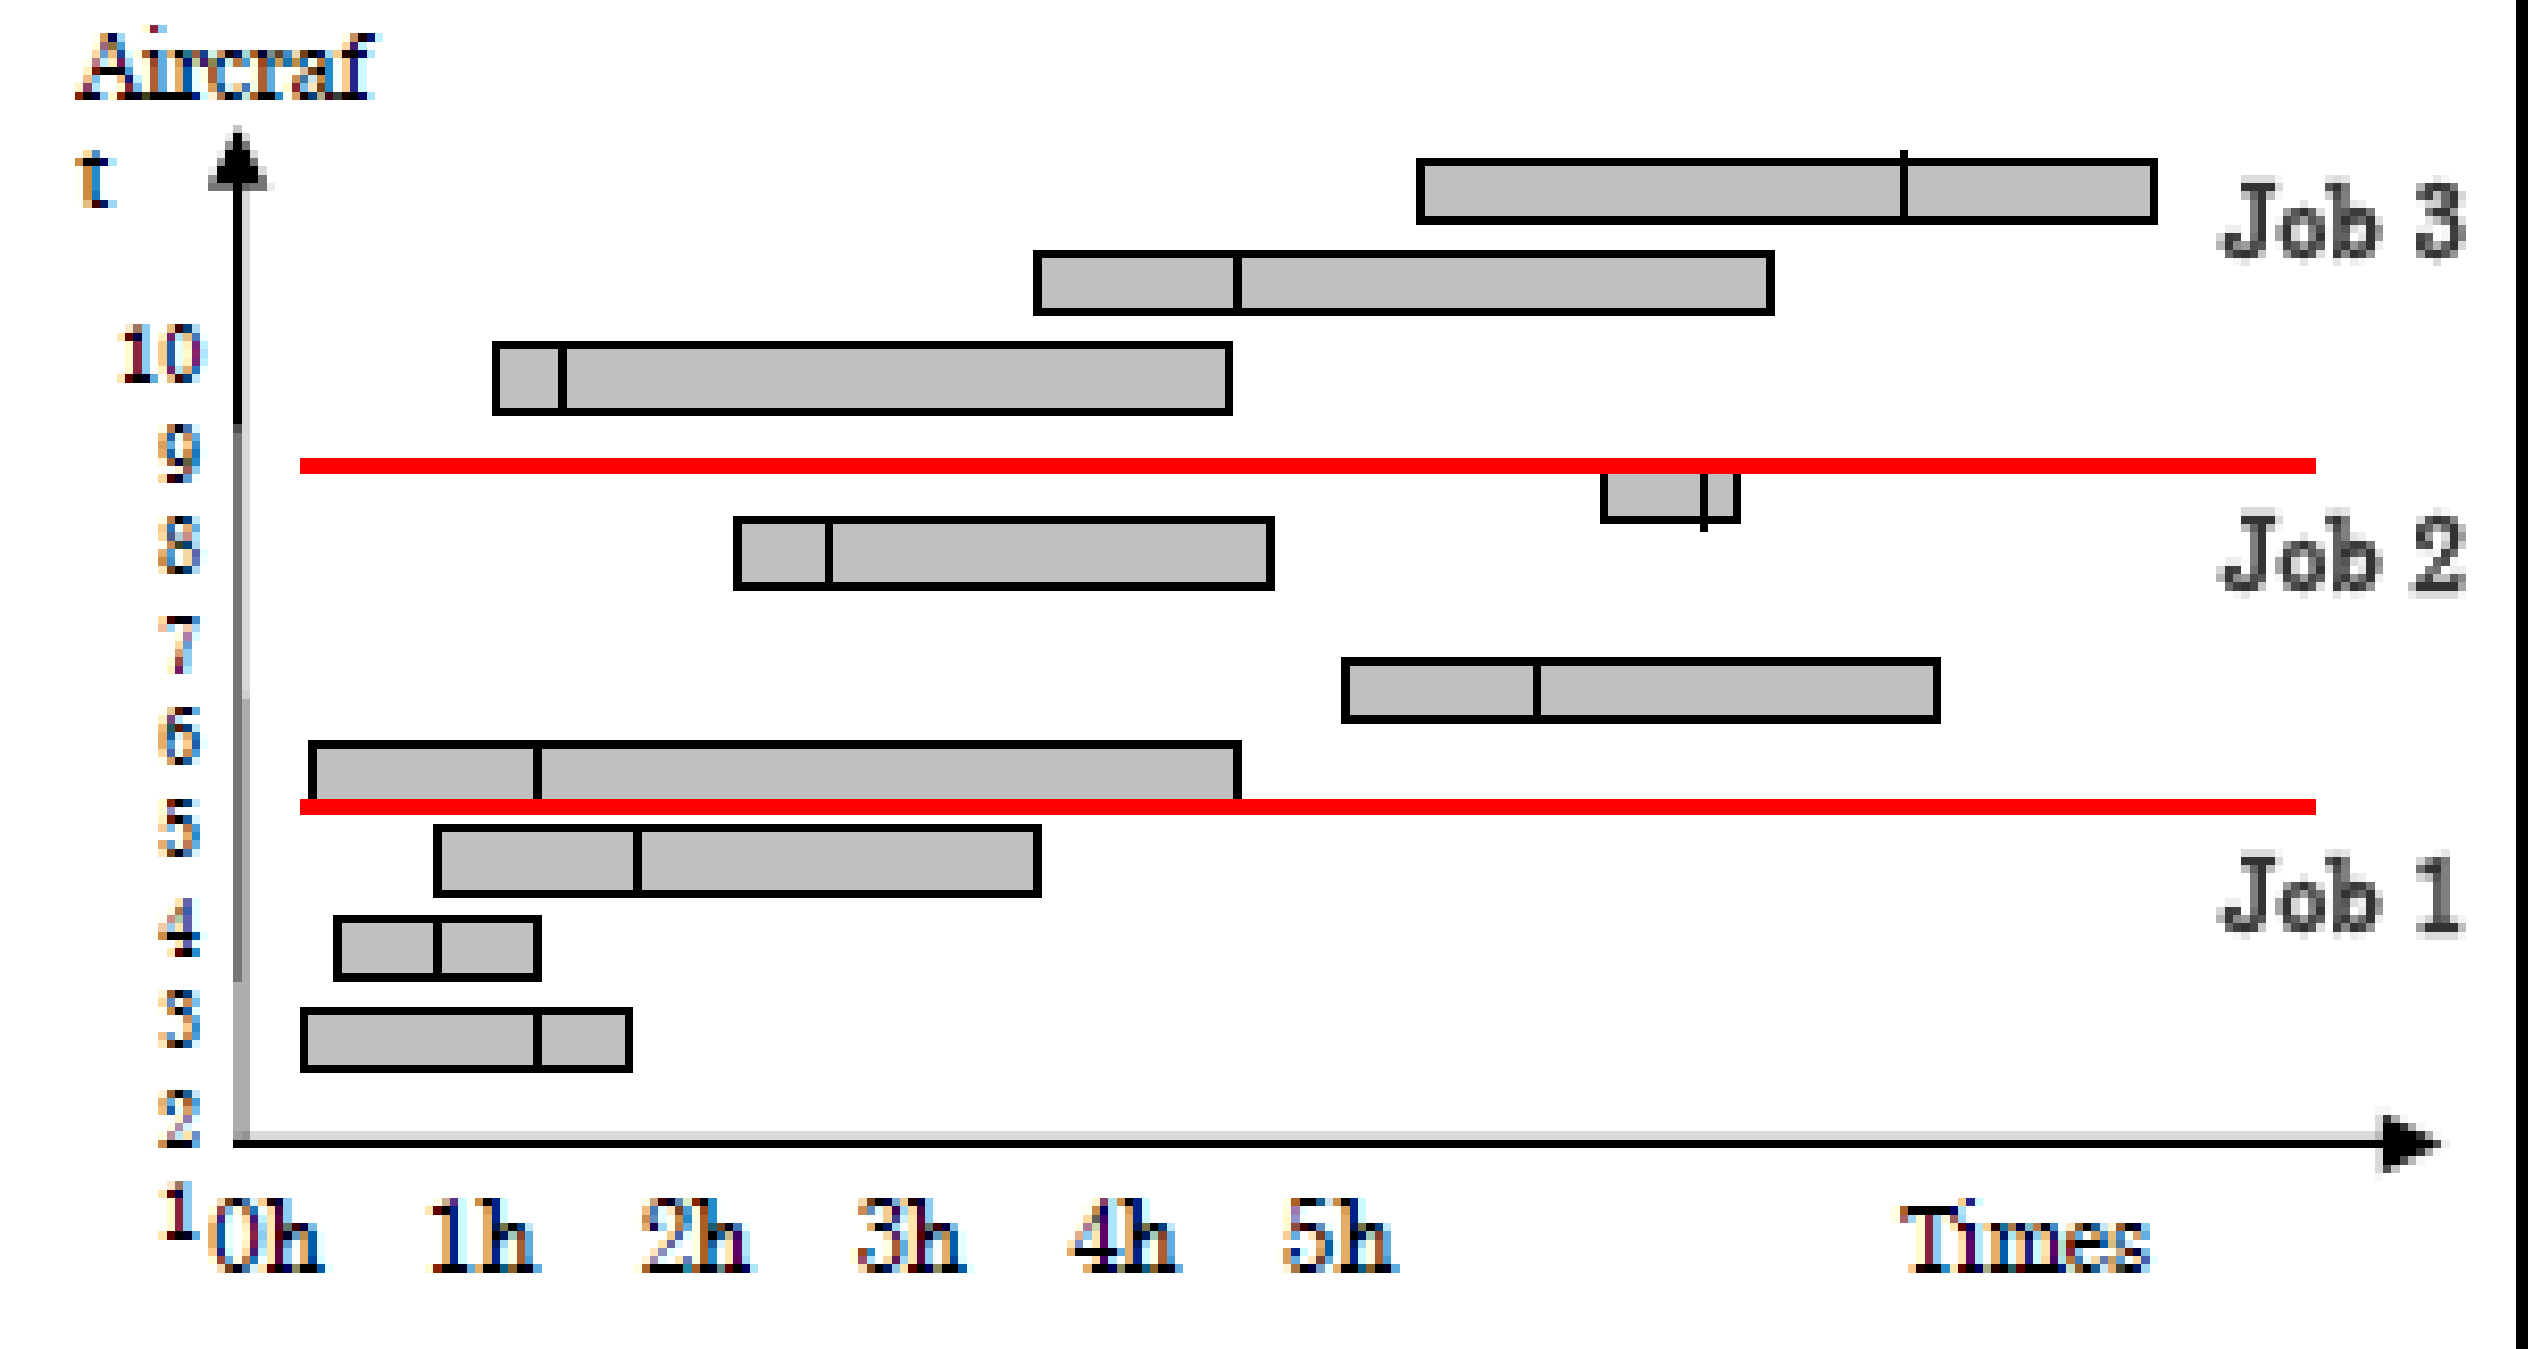
\includegraphics[width=9cm]{job-shop.png}
\centering
\caption{Los aviones se dividen en subconjuntos, llamados Jobs}
\end{figure}

El gran beneficio de este método, es que tiene mucha investigación de respaldo, por lo que sirve para entregar informació valiosa a nuestro ALSP.




\subsection{Tendencia Actual}
Para el ALSP no basta con minimizar los costos, se deben tomar en cuenta todos los factores que pueden influir en el retraso o adelanto de los distintos aterrizajes. Debido a esto los métodos que entregan solo una solución (monosolución), no sirven, ya que se deben considerar multiples alternativas; es aquí donde destacan los algoritmos que utilizan el análisis multiobjetivo gracias a la calidad de sus soluciones.

Pero eso no es todo. Debido a que los algoritmos evolutivos y genéticos tienden a tener tiempos de cómputo más elevados, no siempre resultan como mejor alternativa, dado la necesidad de saber los datos de manera más rápida posible.

Debido a esto, se puede considerar cualquier algoritmo, ya que no existe un algoritmo \textit{mágico}, que sea la mejor opción. Es probable que un algoritmo que sea óptimo en un aeropuerto, no lo sea en otro, debido a las diferencias de tráfico, cantidad de pistas, etc.

\section{Modelo Matem\'atico}
En la sección previa se han expuesto modelos capaces de resolver problemas de ALSP estático e incluso dinámico. Pero para nuestro caso consideraremos solo los ALSP estáticos para $n$ pistas.

Para esto, utilizaremos el método del Job Shop\footnote{JSSP: Job Shop Scheduling Problem}. [3]

\subsection{Variables}
\begin{description}
\item[N:] número de aviones esperando aterrizar.
\item[R:] número de pistas de aterrizaje disponibles.
\item[$e_i$:] el tiempo más temprano de aterrizaje del avión i.
\item[$l_i$:] el tiempo más tarde de aterrizaje del avión i.
\item[$ta_i$:] el tiempo ideal de aterrizaje del avión i.
\item[$Pb_i$:] costo en una unidad de tiempo para avión i adelantado.
\item[$Pa_i$:] costo en una unidad de tiempo para avión i atrasado.
\item[$S_ij$:] ventana de tiempo entre avión i y j, si i aterriza antes de j en la misma pista.
\item[$s_ij$:] ventana de tiempo entre avión i y j, si i aterriza antes de j en distintas pistas. 
\end{description}

\subsection{Variables de decisión}
\begin{description}
\item[$t_i$:] el tiempo calendarizado para el avión i.
\item[$er_i$:]tiempo de adelanto de avión i.
\item[$x_ij$:] 1 si avión i aterriza antes de j, -1 al revés.
\item[$y_ir$:] 1 si avión i aterriza en pista r, 0 si no aterriza en pista r.
\item[$z_ij$:] Si avión i y j aterrizan en la misma pista, 0 si no lo hacen.
\end{description}

\subsection{Restricciones}
\begin{itemize}
\item $e_i\leq t_i\leq l_i$ \textit{el tiempo calendarizado debe estar en la ventana de aterrizaje $[e_i,l_i]$}
\item $X_ij + X_ji = 0$ \textit{i y j no pueden aterrizar juntos}
\item $x_ij * t_j \geq x_ij t_ij + S_ij * z_ij + s_ij(1-z_ij)$ \textit{se debe respetar la separación entre las variables}
\item $\sum\limits_{r=1}^R y_ir = 1$ \textit{un avión solo puede aterrizar en una pista}
\end{itemize}

\subsection{Función Objetivo}
Minimizar el costo de las desviaciones del tiempo real de aterrizaje y el tiempo estimado de aterrizaje.

$Min (\sum\limits_{i=1}^N Pb_i+tr_i * Pa_i)$

\section{Conclusiones}
Dada la gran cantidad de implementación y variaciones de los mismos métodos, existe una amplia gama de alternativas para resolver ALSP, pero por lo general estas son costosas computacionalmente en distintos ámbitos, ya que algoritmos evolutivos entregan soluciones muy interesantes comparadas con las otras, pero recurren en un alto gasto de recursos como la memoria y tiempo de cómputo, y por otro lado, algoritmos que entregan excelentes soluciones óptimas tienen tiempos aún más malos de cómputo. Sin embargo, cada implementación debería ser específica para cada caso, ya que imposible saber a priori como se comportará un algoritmo con ciertos parámetros, por lo que no existe \textit{una gallina de los huevos de oro} que permita el mejor equilibrio.

Dado la corta vida que tiene este tipo de problemas, es importante pensar que la paralelización de estos algoritmos sería una buena opción para acelerar los tiempos de cómputo, en especial en lo de tipo genético, donde se necesita evaluar y comparar distintas opciones no necesariamente en tiempos sincrónicos.

\section{Bibliografía}
A continuación la bibligrafía utilizada para redactar este documento.
\begin{enumerate}
\item An Anytime Algorithm for Scheduling of Aircraft Landing Times Using Genetic Algorithms, Vic Ciesielski, Paul Scerri. Agosto 1998.
\item Scheduling aircraft landings at London Heathrow using a population heuristic, J. E. Beasley, J. Sonander, P. Havelock. Julio 2000.
\item Hybrid method for aircraft landing scheduling based on a Job Shop formulation, G. Bencheikh, J. Boukachour, A. El Hilali Alaoui , and F. El Khoukhi, Agosto 2009
\item Departure Runway Scheduling at London Heathrow Airport Extended Abstract, Jason A. D. Atkin, Edmund K. Burke, John S. Greenwood, Dale Reeson. Octubre 2004..
\item Algorithms of Scheduling Aircraft Landing Problem, Min Wen, Noviembre 2005.
\item Decentralized aircraft landing scheduling at single runway non-controlled airports, Yuanyuan Ding. Mayo 2007.
\item A Multi-objective Evolutionary Approach to Aircraft Landing Scheduling Problems, Ke Tang, Zai Wang, Xianbin Cao, Jun Zhang. 2008
\item Constraint handling based multiobjective evolutionary algorithm for aircraft landing scheduling, Yuanping Guo, Xianbin Cao, Jun Zhang. Junio 2008.
\item Scheduling Aircraft Landings to Balance Workload of Ground Sta, Nils Boysen, Malte Fliedner. Agosto 2008.
\end{enumerate}

\end{document} 
